\begin{center}
    \begin{tabular}{cc}
        % Left Column (Text)
        \begin{minipage}{0.4\linewidth}
            \begin{itemize}
                \item $V_{pp} = 1\text{V}$
                \item $V_{off} = 0.5\text{V}$
                \item $f = 100\text{Hz}$
                \item $R_i = 50\Omega$
            \end{itemize}
        \end{minipage}
         &
        % Right Column (Circuit)
        \begin{minipage}{0.6\linewidth}
            \begin{circuitikz}
                % Draw a voltage source from 0 to 5V
                \draw (0,0) to [sqV, voltage dir=RP, v=$V_{in}$] (0,4);
                \draw (0,4) to [R, l=$100\Omega$] (\linewidth/4,4);
                \draw (\linewidth/4,4) to [L, l=$10\text{mH}$] (\linewidth/2,4);
                % Draw a C that connects to the voltage in
                \draw (\linewidth/2,4) to [C, l=$6\text{n}8\text{F}$] (\linewidth/2,0);
                \draw (\linewidth/2,0) to (0,0);
            \end{circuitikz}
        \end{minipage}
    \end{tabular}
\end{center}

\begin{enumerate}
    \item The function generator was set to produce a 100Hz square wave with an amplitude of $0.5\text{V}$ and an offset of $0.5\text{V}$. It was checked with the oscilloscope if the signal modulated between $0\text{V}$ and $1\text{V}$.

    \item Subsequently, the R-decade was set to $100\Omega$, and the oscilloscope was connected in parallel to the capacitor.

    \item The damped frequency $f_d$ was measured. To determine $f_d$, the period of the exponentially damped sinusoidal waveform was measured using the oscilloscope. A hardcopy was taken of one signal period and another focusing on the ringing phenomenon.
          \begin{figure}[H]
              \centering
              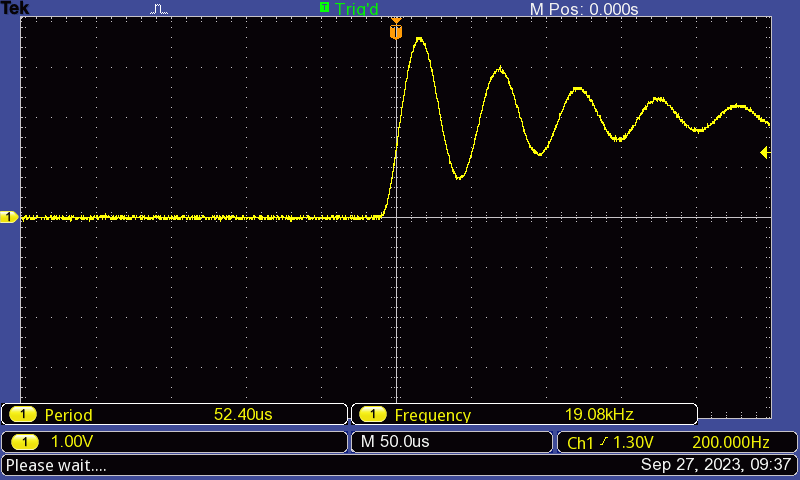
\includegraphics[width=0.8\linewidth]{images/ringing_phenomenon.png}
              \caption{Ringing phenomenon}
              \label{fig:ringing_phenomenon}
          \end{figure}
          According to the figure above, the period of the ringing phenomenon is 52$\mu s$.

    \item Afterward, the damped radian frequency $\omega_d$ was found by knowing that the period of the damped sinusoidal waveform is $f_d = \frac{1}{T}$, where $T=52\mu s$, the period of the ringing phenomenon. Therefore we find that the damped radian frequency $\omega_d$ is
          \begin{equation}
              \begin{gathered}
                  f_d = \frac{1}{T} = \frac{1}{52\mu s} = 1.923 \cdot 10^4 \text{ Hz} \\
                  \omega_d = 2\pi f_d = 1.208 \cdot 10^5 \text{ rad/s}
              \end{gathered}
          \end{equation}
          Very close to the nominal values of
          \begin{equation}
              \begin{gathered}
                  \omega_d = \frac{1}{\sqrt{LC}} = 1.21 \cdot 10^5 \text{ rad/s} \\
                  f_d = \frac{\omega_d}{2\pi} = 1.930 \cdot 10^4 \text{ Hz}
              \end{gathered}
          \end{equation}

    \item The resistance required for the circuit to be critically damped was then calculated.
          \begin{equation}
              \begin{gathered}
                  R = \frac{2\zeta}{\sqrt{C/L}} \implies
                  R_{optimal} = 2\frac{1}{\sqrt{C/L}} - 50\Omega = 2375 \Omega = 2.375 \text{k}\Omega
              \end{gathered}
          \end{equation}
          Where the 50$\Omega$ is subtracted to account for the internal resistance of the function generator.

          \begin{figure}[H]
              \centering
              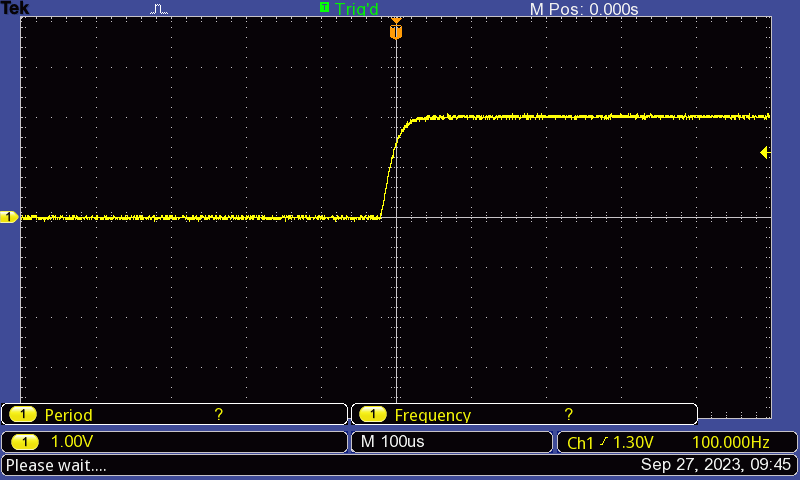
\includegraphics[width=0.8\linewidth]{images/critically_damped_nominal_value.png}
              \caption{Critically damped signal using the nominal resistance value of $2.375\text{k}\Omega$}
              \label{fig:critically_damped_nominal}
          \end{figure}

          However, we find that the optimal resistance is not very close to the nominal value. By playing around with the R-decade, we find that the optimal resistance is
          \begin{equation}
              R_{optimal} = 1905\Omega = 1.905\text{k}\Omega
          \end{equation}

          \begin{figure}[H]
              \centering
              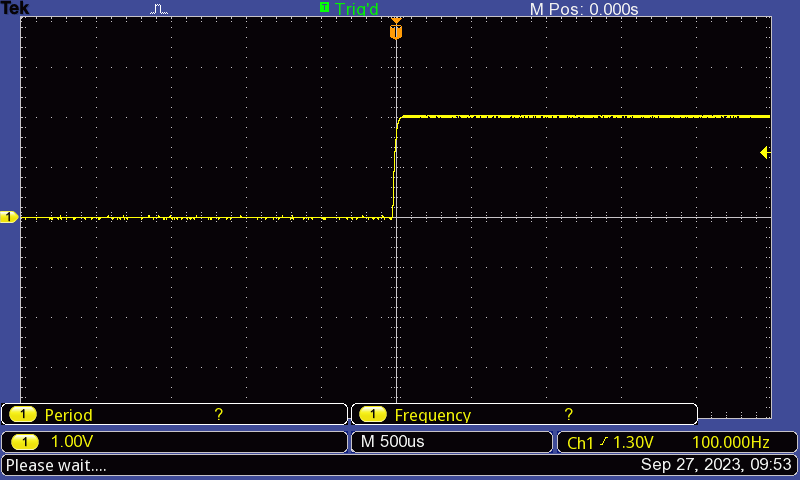
\includegraphics[width=0.6\linewidth]{images/critically_damped.png}
              \caption{Critically damped signal using the tuned resistance value of $1.905\text{k}\Omega$}
              \label{fig:critically_damped_optimal}
          \end{figure}

    \item Finally, the R-decade was set to $30\text{k}\Omega$, causing the circuit to be over-damped. The transient voltage across the capacitor was displayed, and a hardcopy was taken.
          \begin{figure}[H]
              \centering
              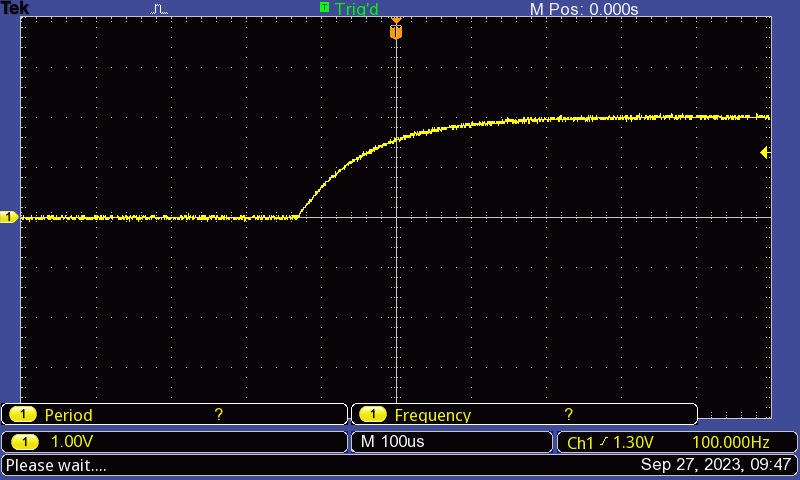
\includegraphics[width=0.6\linewidth]{images/overdamped.png}
              \caption{Over-damped signal}
              \label{fig:over_damped}
          \end{figure}
\end{enumerate}

